% Options for packages loaded elsewhere
\PassOptionsToPackage{unicode}{hyperref}
\PassOptionsToPackage{hyphens}{url}
%
\documentclass[
]{article}
\usepackage{lmodern}
\usepackage{amsmath}
\usepackage{ifxetex,ifluatex}
\ifnum 0\ifxetex 1\fi\ifluatex 1\fi=0 % if pdftex
  \usepackage[T1]{fontenc}
  \usepackage[utf8]{inputenc}
  \usepackage{textcomp} % provide euro and other symbols
  \usepackage{amssymb}
\else % if luatex or xetex
  \usepackage{unicode-math}
  \defaultfontfeatures{Scale=MatchLowercase}
  \defaultfontfeatures[\rmfamily]{Ligatures=TeX,Scale=1}
\fi
% Use upquote if available, for straight quotes in verbatim environments
\IfFileExists{upquote.sty}{\usepackage{upquote}}{}
\IfFileExists{microtype.sty}{% use microtype if available
  \usepackage[]{microtype}
  \UseMicrotypeSet[protrusion]{basicmath} % disable protrusion for tt fonts
}{}
\makeatletter
\@ifundefined{KOMAClassName}{% if non-KOMA class
  \IfFileExists{parskip.sty}{%
    \usepackage{parskip}
  }{% else
    \setlength{\parindent}{0pt}
    \setlength{\parskip}{6pt plus 2pt minus 1pt}}
}{% if KOMA class
  \KOMAoptions{parskip=half}}
\makeatother
\usepackage{xcolor}
\IfFileExists{xurl.sty}{\usepackage{xurl}}{} % add URL line breaks if available
\IfFileExists{bookmark.sty}{\usepackage{bookmark}}{\usepackage{hyperref}}
\hypersetup{
  pdftitle={The  package for data handling, linear estimates and LS-means},
  hidelinks,
  pdfcreator={LaTeX via pandoc}}
\urlstyle{same} % disable monospaced font for URLs
\usepackage[margin=1in]{geometry}
\usepackage{color}
\usepackage{fancyvrb}
\newcommand{\VerbBar}{|}
\newcommand{\VERB}{\Verb[commandchars=\\\{\}]}
\DefineVerbatimEnvironment{Highlighting}{Verbatim}{commandchars=\\\{\}}
% Add ',fontsize=\small' for more characters per line
\usepackage{framed}
\definecolor{shadecolor}{RGB}{248,248,248}
\newenvironment{Shaded}{\begin{snugshade}}{\end{snugshade}}
\newcommand{\AlertTok}[1]{\textcolor[rgb]{0.94,0.16,0.16}{#1}}
\newcommand{\AnnotationTok}[1]{\textcolor[rgb]{0.56,0.35,0.01}{\textbf{\textit{#1}}}}
\newcommand{\AttributeTok}[1]{\textcolor[rgb]{0.77,0.63,0.00}{#1}}
\newcommand{\BaseNTok}[1]{\textcolor[rgb]{0.00,0.00,0.81}{#1}}
\newcommand{\BuiltInTok}[1]{#1}
\newcommand{\CharTok}[1]{\textcolor[rgb]{0.31,0.60,0.02}{#1}}
\newcommand{\CommentTok}[1]{\textcolor[rgb]{0.56,0.35,0.01}{\textit{#1}}}
\newcommand{\CommentVarTok}[1]{\textcolor[rgb]{0.56,0.35,0.01}{\textbf{\textit{#1}}}}
\newcommand{\ConstantTok}[1]{\textcolor[rgb]{0.00,0.00,0.00}{#1}}
\newcommand{\ControlFlowTok}[1]{\textcolor[rgb]{0.13,0.29,0.53}{\textbf{#1}}}
\newcommand{\DataTypeTok}[1]{\textcolor[rgb]{0.13,0.29,0.53}{#1}}
\newcommand{\DecValTok}[1]{\textcolor[rgb]{0.00,0.00,0.81}{#1}}
\newcommand{\DocumentationTok}[1]{\textcolor[rgb]{0.56,0.35,0.01}{\textbf{\textit{#1}}}}
\newcommand{\ErrorTok}[1]{\textcolor[rgb]{0.64,0.00,0.00}{\textbf{#1}}}
\newcommand{\ExtensionTok}[1]{#1}
\newcommand{\FloatTok}[1]{\textcolor[rgb]{0.00,0.00,0.81}{#1}}
\newcommand{\FunctionTok}[1]{\textcolor[rgb]{0.00,0.00,0.00}{#1}}
\newcommand{\ImportTok}[1]{#1}
\newcommand{\InformationTok}[1]{\textcolor[rgb]{0.56,0.35,0.01}{\textbf{\textit{#1}}}}
\newcommand{\KeywordTok}[1]{\textcolor[rgb]{0.13,0.29,0.53}{\textbf{#1}}}
\newcommand{\NormalTok}[1]{#1}
\newcommand{\OperatorTok}[1]{\textcolor[rgb]{0.81,0.36,0.00}{\textbf{#1}}}
\newcommand{\OtherTok}[1]{\textcolor[rgb]{0.56,0.35,0.01}{#1}}
\newcommand{\PreprocessorTok}[1]{\textcolor[rgb]{0.56,0.35,0.01}{\textit{#1}}}
\newcommand{\RegionMarkerTok}[1]{#1}
\newcommand{\SpecialCharTok}[1]{\textcolor[rgb]{0.00,0.00,0.00}{#1}}
\newcommand{\SpecialStringTok}[1]{\textcolor[rgb]{0.31,0.60,0.02}{#1}}
\newcommand{\StringTok}[1]{\textcolor[rgb]{0.31,0.60,0.02}{#1}}
\newcommand{\VariableTok}[1]{\textcolor[rgb]{0.00,0.00,0.00}{#1}}
\newcommand{\VerbatimStringTok}[1]{\textcolor[rgb]{0.31,0.60,0.02}{#1}}
\newcommand{\WarningTok}[1]{\textcolor[rgb]{0.56,0.35,0.01}{\textbf{\textit{#1}}}}
\usepackage{graphicx}
\makeatletter
\def\maxwidth{\ifdim\Gin@nat@width>\linewidth\linewidth\else\Gin@nat@width\fi}
\def\maxheight{\ifdim\Gin@nat@height>\textheight\textheight\else\Gin@nat@height\fi}
\makeatother
% Scale images if necessary, so that they will not overflow the page
% margins by default, and it is still possible to overwrite the defaults
% using explicit options in \includegraphics[width, height, ...]{}
\setkeys{Gin}{width=\maxwidth,height=\maxheight,keepaspectratio}
% Set default figure placement to htbp
\makeatletter
\def\fps@figure{htbp}
\makeatother
\setlength{\emergencystretch}{3em} % prevent overfull lines
\providecommand{\tightlist}{%
  \setlength{\itemsep}{0pt}\setlength{\parskip}{0pt}}
\setcounter{secnumdepth}{-\maxdimen} % remove section numbering
\ifluatex
  \usepackage{selnolig}  % disable illegal ligatures
\fi

\title{The \pkg{doBy} package for data handling, linear estimates and
LS-means}
\author{true}
\date{}

\begin{document}
\maketitle
\begin{abstract}
The \pkg{doBy} is one of several general utility packages on CRAN. We
illustrate two main features of the package: The ability to making
groupwise computations and the ability to compute linear estimates,
contrasts and least-squares means.
\end{abstract}

\hypertarget{introduction}{%
\subsection{Introduction}\label{introduction}}

The \CRANpkg{doBy} package {[}@doby{]} grew out of a need to calculate
groupwise summary statistics (much in the spirit of \code{PROC SUMMARY}
of the SAS system, {[}@procsummary{]}). The package first appeared on
CRAN, \url{https://cran-r-project.org}, in 2006. The name \pkg{doBy}
comes from the need to \textbf{do} some computations on data which is
stratified \textbf{By} the value of some variables. Today the package
contains many additional utilities. In this paper we focus 1) on the
``doing by''-functions and 2) on functions related to linear estimates
and contrasts (in particular LS-means).

\hypertarget{related-functionality}{%
\subsubsection{Related functionality}\label{related-functionality}}

When it comes to data handling, \pkg{doBy} is nowhere nearly as powerful
as more contemporary packages, such as those in the \CRANpkg{tidyverse}
eco system, {[}@tidyverse{]}. The \code{aggregate} function in base R
provides functionality similar to \pkg{doBy}s \code{summaryBy} function.
Another package to be mentioned in this connection is
\CRANpkg{data.table}, @data.table. On the other hand, \pkg{doBy} is
based on classical data structures that are unlikely to undergo sudden
changes. There is one exception to this, though: The data handling
functions work on tibble`s, from \CRANpkg{tibble} @tibble. In relation
to linear estimates, the \CRANpkg{multcomp} package {[}@multcomp{]}
deserves mention, and the \CRANpkg{lsmeans} package {[}@lsmeans{]}
provides facilities for computing LS-means.

It can be hypothesized that the data handling functions in \pkg{doBy}
remain appealing to a group of users because of their simplicity.

\hypertarget{a-working-dataset---the-co2-data}{%
\subsubsection{\texorpdfstring{A working dataset - the \texttt{CO2}
data}{A working dataset - the CO2 data}}\label{a-working-dataset---the-co2-data}}

The \texttt{CO2} data frame comes from an experiment on the cold
tolerance of the grass species \emph{Echinochloa crus-galli}.
\texttt{Type} is a factor with levels \texttt{Quebec} or
\texttt{Mississippi} giving the origin of the plant. \texttt{Treatment}
is a factor levels \texttt{nonchilled} or \texttt{chilled}. Data is
balanced with respect to these two factors. However, illustrated certain
points we exclude a few rows of data to make data imbalanced. To limit
the amount of output we modify names and levels of variables as follows

\begin{Shaded}
\begin{Highlighting}[]
\FunctionTok{data}\NormalTok{(CO2)}
\NormalTok{CO2 }\OtherTok{\textless{}{-}} \FunctionTok{within}\NormalTok{(CO2, \{}
\NormalTok{    Treat }\OtherTok{=}\NormalTok{ Treatment; Treatment }\OtherTok{=} \ConstantTok{NULL}
    \FunctionTok{levels}\NormalTok{(Treat) }\OtherTok{=} \FunctionTok{c}\NormalTok{(}\StringTok{"nchil"}\NormalTok{, }\StringTok{"chil"}\NormalTok{); }\FunctionTok{levels}\NormalTok{(Type) }\OtherTok{=} \FunctionTok{c}\NormalTok{(}\StringTok{"Que"}\NormalTok{, }\StringTok{"Mis"}\NormalTok{)}
\NormalTok{\})}
\NormalTok{CO2 }\OtherTok{\textless{}{-}} \FunctionTok{subset}\NormalTok{(CO2, Plant }\SpecialCharTok{\%in\%} \FunctionTok{c}\NormalTok{(}\StringTok{"Qn1"}\NormalTok{, }\StringTok{"Qc1"}\NormalTok{, }\StringTok{"Mn1"}\NormalTok{, }\StringTok{"Mc1"}\NormalTok{))}
\NormalTok{CO2 }\OtherTok{\textless{}{-}}\NormalTok{ CO2[}\SpecialCharTok{{-}}\NormalTok{(}\DecValTok{1}\SpecialCharTok{:}\DecValTok{3}\NormalTok{),]}
\FunctionTok{xtabs}\NormalTok{(}\SpecialCharTok{\textasciitilde{}}\NormalTok{Treat}\SpecialCharTok{+}\NormalTok{Type, }\AttributeTok{data=}\NormalTok{CO2)}
\end{Highlighting}
\end{Shaded}

\begin{verbatim}
##        Type
## Treat   Que Mis
##   nchil   4   7
##   chil    7   7
\end{verbatim}

\begin{Shaded}
\begin{Highlighting}[]
\FunctionTok{head}\NormalTok{(CO2, }\DecValTok{4}\NormalTok{)}
\end{Highlighting}
\end{Shaded}

\begin{verbatim}
##   Plant Type conc uptake Treat
## 4   Qn1  Que  350   37.2 nchil
## 5   Qn1  Que  500   35.3 nchil
## 6   Qn1  Que  675   39.2 nchil
## 7   Qn1  Que 1000   39.7 nchil
\end{verbatim}

\begin{figure}
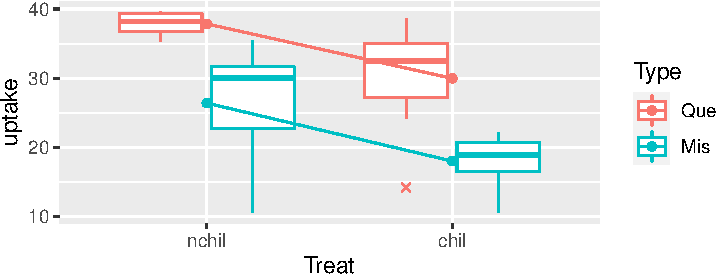
\includegraphics[keepaspectratio]{doby-hojsgaard-fig-interaction-1} \caption{Interaction plot for the CO2 data. Boxplot outliers are crosses. The plot suggests additivity between Treat and Type.}\label{fig:interaction}
\end{figure}

\hypertarget{functions-related-to-groupwise-computations}{%
\subsection{Functions related to groupwise
computations}\label{functions-related-to-groupwise-computations}}

\hypertarget{the-function}{%
\subsubsection{\texorpdfstring{The \code{summaryBy}
function}{The  function}}\label{the-function}}

The \code{summaryBy} function is used for calculating quantities like
\emph{the mean and variance of numerical variables x and y for each
combination of two factors A and B}. Notice: A functionality similar to
\code{summaryBy} is provided by \code{aggregate} from base R, but
\code{summaryBy} offers additional features.

\begin{Shaded}
\begin{Highlighting}[]
\NormalTok{myfun1 }\OtherTok{\textless{}{-}} \ControlFlowTok{function}\NormalTok{(x)\{}\FunctionTok{c}\NormalTok{(}\AttributeTok{m=}\FunctionTok{mean}\NormalTok{(x), }\AttributeTok{s=}\FunctionTok{sd}\NormalTok{(x))\}}
\FunctionTok{summaryBy}\NormalTok{(}\FunctionTok{cbind}\NormalTok{(conc, uptake, }\AttributeTok{lu=}\FunctionTok{log}\NormalTok{(uptake)) }\SpecialCharTok{\textasciitilde{}}\NormalTok{ Plant, }\AttributeTok{data=}\NormalTok{CO2, }\AttributeTok{FUN=}\NormalTok{myfun1)}
\end{Highlighting}
\end{Shaded}

\begin{verbatim}
##   Plant conc.m conc.s uptake.m uptake.s  lu.m    lu.s
## 1   Qn1  631.2  279.4    37.85    2.014 3.633 0.05375
## 2   Qc1  435.0  317.7    29.97    8.335 3.356 0.34457
## 3   Mn1  435.0  317.7    26.40    8.694 3.209 0.42341
## 4   Mc1  435.0  317.7    18.00    4.119 2.864 0.26219
\end{verbatim}

The convention is that variables that do not appear in the dataframe
(e.g.~\code{log(uptake)}) must be named (here as \code{lu}). Various
shortcuts are available, e.g.~the following, where left hand side dot
refers to \emph{all numeric variables} while the right hand side dot
refers to \emph{all factor variables}. Writing \texttt{1} on the right
hand side leads to computing over the entire dataset:

\begin{Shaded}
\begin{Highlighting}[]
\FunctionTok{summaryBy}\NormalTok{(. }\SpecialCharTok{\textasciitilde{}}\NormalTok{ ., }\AttributeTok{data=}\NormalTok{CO2, }\AttributeTok{FUN=}\NormalTok{myfun1)}
\end{Highlighting}
\end{Shaded}

\begin{verbatim}
##   Plant Type Treat conc.m conc.s uptake.m uptake.s
## 1   Qn1  Que nchil  631.2  279.4    37.85    2.014
## 2   Qc1  Que  chil  435.0  317.7    29.97    8.335
## 3   Mn1  Mis nchil  435.0  317.7    26.40    8.694
## 4   Mc1  Mis  chil  435.0  317.7    18.00    4.119
\end{verbatim}

\begin{Shaded}
\begin{Highlighting}[]
\FunctionTok{summaryBy}\NormalTok{(. }\SpecialCharTok{\textasciitilde{}} \DecValTok{1}\NormalTok{, }\AttributeTok{data=}\NormalTok{CO2, }\AttributeTok{FUN=}\NormalTok{myfun1)}
\end{Highlighting}
\end{Shaded}

\begin{verbatim}
##   conc.m conc.s uptake.m uptake.s
## 1  466.4  301.4    26.88    9.323
\end{verbatim}

\hypertarget{specifications-as-formulas-and-lists}{%
\subsubsection{Specifications as formulas and
lists}\label{specifications-as-formulas-and-lists}}

We shall refer to all the functions for groupwise computations etc. as
the \emph{By-functions}. The convention for the By-functions is that a
two sided formula like can be written in two ways:

\begin{Shaded}
\begin{Highlighting}[]
\FunctionTok{cbind}\NormalTok{(x, y) }\SpecialCharTok{\textasciitilde{}}\NormalTok{ A }\SpecialCharTok{+}\NormalTok{ B}
\FunctionTok{list}\NormalTok{(}\FunctionTok{c}\NormalTok{(}\StringTok{"x"}\NormalTok{, }\StringTok{"y"}\NormalTok{), }\FunctionTok{c}\NormalTok{(}\StringTok{"A"}\NormalTok{, }\StringTok{"B"}\NormalTok{))}
\end{Highlighting}
\end{Shaded}

Some By-functions only take a right hand sided formula as input. Such a
formula can also be written in two ways:

\begin{Shaded}
\begin{Highlighting}[]
\SpecialCharTok{\textasciitilde{}}\NormalTok{ A }\SpecialCharTok{+}\NormalTok{ B}
\FunctionTok{c}\NormalTok{(}\StringTok{"A"}\NormalTok{, }\StringTok{"B"}\NormalTok{)}
\end{Highlighting}
\end{Shaded}

The list-form / vector-form is especially useful if a function is
invoked programatically. Hence the calls to \code{summaryBy} above can
also be made as

\begin{Shaded}
\begin{Highlighting}[]
\FunctionTok{summaryBy}\NormalTok{(}\FunctionTok{list}\NormalTok{(}\FunctionTok{c}\NormalTok{(}\StringTok{"conc"}\NormalTok{, }\StringTok{"uptake"}\NormalTok{, }\StringTok{"lu=log(uptake)"}\NormalTok{), }\StringTok{"Plant"}\NormalTok{), }\AttributeTok{data=}\NormalTok{CO2, }\AttributeTok{FUN=}\NormalTok{myfun1)}
\FunctionTok{summaryBy}\NormalTok{(}\FunctionTok{list}\NormalTok{(}\StringTok{"."}\NormalTok{, }\StringTok{"."}\NormalTok{), }\AttributeTok{data=}\NormalTok{CO2, }\AttributeTok{FUN=}\NormalTok{myfun1)}
\FunctionTok{summaryBy}\NormalTok{(}\FunctionTok{list}\NormalTok{(}\StringTok{"."}\NormalTok{, }\StringTok{"1"}\NormalTok{), }\AttributeTok{data=}\NormalTok{CO2, }\AttributeTok{FUN=}\NormalTok{myfun1)}
\end{Highlighting}
\end{Shaded}

\hypertarget{using-the-pipe-operator}{%
\subsection{Using the pipe operator}\label{using-the-pipe-operator}}

The \code{summaryBy} function has a counterpart called
\code{summary\_by}. The difference is that a formula is the first
argument to the former function while a dataframe (or a tibble) is the
first argument to the latter. The same applies to the other
By-functions. This allows for elegant use of the pipe operator
\texttt{\%\textgreater{}\%} from \CRANpkg{magrittr}, {[}@magrittr{]}:

\begin{Shaded}
\begin{Highlighting}[]
\NormalTok{CO2 }\SpecialCharTok{\%\textgreater{}\%} \FunctionTok{summary\_by}\NormalTok{(}\FunctionTok{cbind}\NormalTok{(conc, uptake) }\SpecialCharTok{\textasciitilde{}}\NormalTok{ Plant }\SpecialCharTok{+}\NormalTok{ Type, }\AttributeTok{FUN=}\NormalTok{myfun1) }\OtherTok{{-}\textgreater{}}\NormalTok{ newdat}
\NormalTok{newdat}
\end{Highlighting}
\end{Shaded}

\begin{verbatim}
##   Plant Type conc.m conc.s uptake.m uptake.s
## 1   Qn1  Que  631.2  279.4    37.85    2.014
## 2   Qc1  Que  435.0  317.7    29.97    8.335
## 3   Mn1  Mis  435.0  317.7    26.40    8.694
## 4   Mc1  Mis  435.0  317.7    18.00    4.119
\end{verbatim}

\hypertarget{the-function-1}{%
\subsubsection{\texorpdfstring{The \code{orderBy}
function}{The  function}}\label{the-function-1}}

Ordering (or sorting) a data frame is possible with the \texttt{orderBy}
function. Suppose we want to order the rows of the the \texttt{CO2} data
by increasing values of \texttt{conc} and decreasing value of
\texttt{uptake} (within \texttt{conc}):

\begin{Shaded}
\begin{Highlighting}[]
\NormalTok{x1 }\OtherTok{\textless{}{-}} \FunctionTok{orderBy}\NormalTok{(}\SpecialCharTok{\textasciitilde{}}\NormalTok{ conc }\SpecialCharTok{{-}}\NormalTok{ uptake, }\AttributeTok{data=}\NormalTok{CO2)}
\FunctionTok{head}\NormalTok{(x1)}
\end{Highlighting}
\end{Shaded}

\begin{verbatim}
##    Plant Type conc uptake Treat
## 22   Qc1  Que   95   14.2  chil
## 43   Mn1  Mis   95   10.6 nchil
## 64   Mc1  Mis   95   10.5  chil
## 23   Qc1  Que  175   24.1  chil
## 44   Mn1  Mis  175   19.2 nchil
## 65   Mc1  Mis  175   14.9  chil
\end{verbatim}

\hypertarget{the-function-2}{%
\subsubsection{\texorpdfstring{The \code{splitBy}
function}{The  function}}\label{the-function-2}}

Suppose we want to split \texttt{CO2} into a list of dataframes:

\begin{Shaded}
\begin{Highlighting}[]
\NormalTok{x1 }\OtherTok{\textless{}{-}} \FunctionTok{splitBy}\NormalTok{(}\SpecialCharTok{\textasciitilde{}}\NormalTok{ Plant }\SpecialCharTok{+}\NormalTok{ Type, }\AttributeTok{data=}\NormalTok{CO2)}
\NormalTok{x1}
\end{Highlighting}
\end{Shaded}

\begin{verbatim}
##   listentry Plant Type
## 1   Qn1|Que   Qn1  Que
## 2   Qc1|Que   Qc1  Que
## 3   Mn1|Mis   Mn1  Mis
## 4   Mc1|Mis   Mc1  Mis
\end{verbatim}

The result is a list (with a few additional attributes):

\begin{Shaded}
\begin{Highlighting}[]
\FunctionTok{lapply}\NormalTok{(x1, head, }\DecValTok{2}\NormalTok{)}
\end{Highlighting}
\end{Shaded}

\begin{verbatim}
## $`Qn1|Que`
##   Plant Type conc uptake Treat
## 4   Qn1  Que  350   37.2 nchil
## 5   Qn1  Que  500   35.3 nchil
## 
## $`Qc1|Que`
##    Plant Type conc uptake Treat
## 22   Qc1  Que   95   14.2  chil
## 23   Qc1  Que  175   24.1  chil
## 
## $`Mn1|Mis`
##    Plant Type conc uptake Treat
## 43   Mn1  Mis   95   10.6 nchil
## 44   Mn1  Mis  175   19.2 nchil
## 
## $`Mc1|Mis`
##    Plant Type conc uptake Treat
## 64   Mc1  Mis   95   10.5  chil
## 65   Mc1  Mis  175   14.9  chil
\end{verbatim}

\hypertarget{the-function-3}{%
\subsubsection{\texorpdfstring{The \code{subsetBy}
function}{The  function}}\label{the-function-3}}

Suppose we want to select those rows within each treatment for which the
uptake is larger than 75\% quantile of uptake (within the treatment).
This is achieved by:

\begin{Shaded}
\begin{Highlighting}[]
\NormalTok{x2 }\OtherTok{\textless{}{-}} \FunctionTok{subsetBy}\NormalTok{(}\SpecialCharTok{\textasciitilde{}}\NormalTok{ Treat, }\AttributeTok{subset=}\NormalTok{uptake }\SpecialCharTok{\textgreater{}} \FunctionTok{quantile}\NormalTok{(uptake, }\AttributeTok{prob=}\FloatTok{0.75}\NormalTok{), }\AttributeTok{data=}\NormalTok{CO2)}
\FunctionTok{head}\NormalTok{(x2, }\DecValTok{4}\NormalTok{)}
\end{Highlighting}
\end{Shaded}

\begin{verbatim}
##         Plant Type conc uptake Treat
## nchil.4   Qn1  Que  350   37.2 nchil
## nchil.6   Qn1  Que  675   39.2 nchil
## nchil.7   Qn1  Que 1000   39.7 nchil
## chil.25   Qc1  Que  350   34.6  chil
\end{verbatim}

\hypertarget{the-function-4}{%
\subsubsection{\texorpdfstring{The \code{transformBy}
function}{The  function}}\label{the-function-4}}

The \code{transformBy} function is analogous to the \code{transform}
function except that it works within groups. For example:

\begin{Shaded}
\begin{Highlighting}[]
\NormalTok{x3 }\OtherTok{\textless{}{-}} \FunctionTok{transformBy}\NormalTok{(}\SpecialCharTok{\textasciitilde{}}\NormalTok{ Treat, }\AttributeTok{data=}\NormalTok{CO2, }
                 \AttributeTok{minU=}\FunctionTok{min}\NormalTok{(uptake), }\AttributeTok{maxU=}\FunctionTok{max}\NormalTok{(uptake), }\AttributeTok{range=}\FunctionTok{diff}\NormalTok{(}\FunctionTok{range}\NormalTok{(uptake)))}
\FunctionTok{head}\NormalTok{(x3, }\DecValTok{4}\NormalTok{)}
\end{Highlighting}
\end{Shaded}

\begin{verbatim}
##   Plant Type conc uptake Treat minU maxU range
## 1   Qn1  Que  350   37.2 nchil 10.6 39.7  29.1
## 2   Qn1  Que  500   35.3 nchil 10.6 39.7  29.1
## 3   Qn1  Que  675   39.2 nchil 10.6 39.7  29.1
## 4   Qn1  Que 1000   39.7 nchil 10.6 39.7  29.1
\end{verbatim}

\hypertarget{the-function-5}{%
\subsubsection{\texorpdfstring{The \code{lmBy}
function}{The  function}}\label{the-function-5}}

The \code{lmBy} function allows for fitting linear models to different
strata of data (the vertical bar is used for defining groupings of
data):

\begin{Shaded}
\begin{Highlighting}[]
\NormalTok{m }\OtherTok{\textless{}{-}} \FunctionTok{lmBy}\NormalTok{(uptake }\SpecialCharTok{\textasciitilde{}}\NormalTok{ conc }\SpecialCharTok{|}\NormalTok{ Treat, }\AttributeTok{data=}\NormalTok{CO2)}
\FunctionTok{coef}\NormalTok{(m)}
\end{Highlighting}
\end{Shaded}

\begin{verbatim}
##       (Intercept)    conc
## nchil       19.32 0.02221
## chil        17.02 0.01602
\end{verbatim}

The result is a list with a few additional attributes and the list can
be processed further as e.g.

\begin{Shaded}
\begin{Highlighting}[]
\FunctionTok{lapply}\NormalTok{(m, }\ControlFlowTok{function}\NormalTok{(z) }\FunctionTok{coef}\NormalTok{(}\FunctionTok{summary}\NormalTok{(z)))}
\end{Highlighting}
\end{Shaded}

\begin{verbatim}
## $nchil
##             Estimate Std. Error t value  Pr(>|t|)
## (Intercept) 19.31969   3.692936   5.232 0.0005408
## conc         0.02221   0.006318   3.515 0.0065698
## 
## $chil
##             Estimate Std. Error t value  Pr(>|t|)
## (Intercept) 17.01814   3.668315   4.639 0.0005709
## conc         0.01602   0.006986   2.293 0.0407168
\end{verbatim}

\hypertarget{functions-related-linear-estimates-and-contrasts}{%
\subsection{Functions related linear estimates and
contrasts}\label{functions-related-linear-estimates-and-contrasts}}

A linear function of a \(p\)--dimensional parameter vector \(\beta\) has
the form \begin{displaymath}
  C=L\beta
\end{displaymath} where \(L\) is a \(q\times p\) matrix which we call
the \emph{Linear Estimate Matrix} or simply \emph{LE-matrix}. The
corresponding linear estimate is \(\hat C = L \hat \beta\). A linear
hypothesis has the form \(H_0: L\beta=m\) for some \(q\) dimensional
vector \(m\).

In the following we describe what is essentially simple ways of
generating such \(L\)-matrices.

\hypertarget{computing-linear-estimates}{%
\subsubsection{Computing linear
estimates}\label{computing-linear-estimates}}

First we focus on an additive model.

\begin{Shaded}
\begin{Highlighting}[]
\NormalTok{co2.add }\OtherTok{\textless{}{-}} \FunctionTok{lm}\NormalTok{(uptake }\SpecialCharTok{\textasciitilde{}}\NormalTok{ Treat }\SpecialCharTok{+}\NormalTok{ Type, }\AttributeTok{data=}\NormalTok{CO2)}
\end{Highlighting}
\end{Shaded}

Consider computing the estimated uptake for each treatment for plants
originating from Mississippi: One option: Construct the LE--matrix \(L\)
directly and then compute \(L\hat\beta\):

\begin{Shaded}
\begin{Highlighting}[]
\NormalTok{L }\OtherTok{\textless{}{-}} \FunctionTok{matrix}\NormalTok{(}\FunctionTok{c}\NormalTok{(}\DecValTok{1}\NormalTok{, }\DecValTok{0}\NormalTok{, }\DecValTok{1}\NormalTok{, }
              \DecValTok{1}\NormalTok{, }\DecValTok{1}\NormalTok{, }\DecValTok{1}\NormalTok{), }\AttributeTok{nrow=}\DecValTok{2}\NormalTok{, }\AttributeTok{byrow=}\NormalTok{T); L}
\end{Highlighting}
\end{Shaded}

\begin{verbatim}
##      [,1] [,2] [,3]
## [1,]    1    0    1
## [2,]    1    1    1
\end{verbatim}

\begin{Shaded}
\begin{Highlighting}[]
\NormalTok{beta }\OtherTok{\textless{}{-}} \FunctionTok{coef}\NormalTok{(co2.add); beta}
\end{Highlighting}
\end{Shaded}

\begin{verbatim}
## (Intercept)   Treatchil     TypeMis 
##       38.04       -8.18      -11.75
\end{verbatim}

\begin{Shaded}
\begin{Highlighting}[]
\NormalTok{L }\SpecialCharTok{\%*\%}\NormalTok{ beta}
\end{Highlighting}
\end{Shaded}

\begin{verbatim}
##       [,1]
## [1,] 26.29
## [2,] 18.11
\end{verbatim}

However, this approach does not produce standard errors, confidence
intervals etc. Once \(L\) has been constructed, such quantities can be
constructed using \code{linest} (short for \emph{linear estimate}) and
the older but very similar \code{esticon} function (short for
\emph{estimate contrast})

\begin{Shaded}
\begin{Highlighting}[]
\NormalTok{c1 }\OtherTok{\textless{}{-}} \FunctionTok{linest}\NormalTok{(co2.add, L)}
\FunctionTok{coef}\NormalTok{(c1)}
\end{Highlighting}
\end{Shaded}

\begin{verbatim}
##   estimate std.error statistic df   p.value
## 1    26.29     2.247     11.70 22 6.440e-11
## 2    18.11     2.247      8.06 22 5.209e-08
\end{verbatim}

\begin{Shaded}
\begin{Highlighting}[]
\FunctionTok{confint}\NormalTok{(c1)}
\end{Highlighting}
\end{Shaded}

\begin{verbatim}
##   0.025 0.975
## 1 21.63 30.95
## 2 13.45 22.77
\end{verbatim}

\begin{Shaded}
\begin{Highlighting}[]
\NormalTok{c1 }\OtherTok{\textless{}{-}} \FunctionTok{esticon}\NormalTok{(co2.add, L)}
\NormalTok{c1}
\end{Highlighting}
\end{Shaded}

\begin{verbatim}
##      estimate std.error statistic  p.value    beta0 df
## [1,] 2.63e+01  2.25e+00  1.17e+01 6.44e-11 0.00e+00 22
## [2,] 1.81e+01  2.25e+00  8.06e+00 5.21e-08 0.00e+00 22
\end{verbatim}

Another option is to invoke \code{glht} (short for \emph{general linear
hypothesis}) from the \CRANpkg{multcomp} package:

\begin{Shaded}
\begin{Highlighting}[]
\FunctionTok{library}\NormalTok{(multcomp)}
\NormalTok{mc }\OtherTok{\textless{}{-}} \FunctionTok{glht}\NormalTok{(co2.add, }\AttributeTok{linfct=}\NormalTok{L)}
\FunctionTok{summary}\NormalTok{(mc)}
\end{Highlighting}
\end{Shaded}

\begin{verbatim}
## 
##   Simultaneous Tests for General Linear Hypotheses
## 
## Fit: lm(formula = uptake ~ Treat + Type, data = CO2)
## 
## Linear Hypotheses:
##        Estimate Std. Error t value Pr(>|t|)
## 1 == 0    26.29       2.25   11.70  1.3e-10
## 2 == 0    18.11       2.25    8.06  1.0e-07
## (Adjusted p values reported -- single-step method)
\end{verbatim}

In \pkg{doBy} there are facilities for computing \(L\) automatically and
for supplying \(L\hat\beta\) with standard errors etc.

\begin{Shaded}
\begin{Highlighting}[]
\NormalTok{L }\OtherTok{\textless{}{-}} \FunctionTok{LE\_matrix}\NormalTok{(co2.add, }\AttributeTok{effect =} \StringTok{"Treat"}\NormalTok{, }\AttributeTok{at=}\FunctionTok{list}\NormalTok{(}\AttributeTok{Type=}\StringTok{"Mis"}\NormalTok{)); L}
\end{Highlighting}
\end{Shaded}

\begin{verbatim}
##      (Intercept) Treatchil TypeMis
## [1,]           1         0       1
## [2,]           1         1       1
\end{verbatim}

\hypertarget{least-squares-means-lsmeans}{%
\subsubsection{Least-squares means
(LS--means)}\label{least-squares-means-lsmeans}}

A related question is: What is the estimated uptake for each treatment
if we ignore the type (i.e.~origin of the plants)? One option would to
fit a linear model without \texttt{Type} as explanatory variable:

\begin{Shaded}
\begin{Highlighting}[]
\NormalTok{co2}\FloatTok{.0} \OtherTok{\textless{}{-}} \FunctionTok{update}\NormalTok{(co2.add, . }\SpecialCharTok{\textasciitilde{}}\NormalTok{ . }\SpecialCharTok{{-}}\NormalTok{ Type)}
\NormalTok{L0 }\OtherTok{\textless{}{-}} \FunctionTok{LE\_matrix}\NormalTok{(co2}\FloatTok{.0}\NormalTok{, }\AttributeTok{effect=}\StringTok{"Treat"}\NormalTok{); L0}
\end{Highlighting}
\end{Shaded}

\begin{verbatim}
##      (Intercept) Treatchil
## [1,]           1         0
## [2,]           1         1
\end{verbatim}

\begin{Shaded}
\begin{Highlighting}[]
\FunctionTok{linest}\NormalTok{(co2}\FloatTok{.0}\NormalTok{, }\AttributeTok{L=}\NormalTok{L0)}
\end{Highlighting}
\end{Shaded}

\begin{verbatim}
## Coefficients:
##      estimate std.error statistic    df p.value
## [1,]    30.56      2.68     11.40 23.00       0
## [2,]    23.99      2.38     10.09 23.00       0
\end{verbatim}

An alternative would be to keep the focus on the original model but
compute the estimated uptake for each treatment for an \emph{average
location}. That would correspond to giving weight \(1/2\) to each of the
two locations. However, as one of the parameters is already set to zero
to obtain identifiability, we obtain the LE--matrix \(L\) as

\begin{Shaded}
\begin{Highlighting}[]
\NormalTok{L1 }\OtherTok{\textless{}{-}} \FunctionTok{matrix}\NormalTok{(}\FunctionTok{c}\NormalTok{(}\DecValTok{1}\NormalTok{, }\DecValTok{0}\NormalTok{, }\FloatTok{0.5}\NormalTok{, }
               \DecValTok{1}\NormalTok{, }\DecValTok{1}\NormalTok{, }\FloatTok{0.5}\NormalTok{), }\AttributeTok{nrow=}\DecValTok{2}\NormalTok{, }\AttributeTok{byrow=}\NormalTok{T); L1}
\end{Highlighting}
\end{Shaded}

\begin{verbatim}
##      [,1] [,2] [,3]
## [1,]    1    0  0.5
## [2,]    1    1  0.5
\end{verbatim}

\begin{Shaded}
\begin{Highlighting}[]
\FunctionTok{linest}\NormalTok{(co2.add, }\AttributeTok{L=}\NormalTok{L1)}
\end{Highlighting}
\end{Shaded}

\begin{verbatim}
## Coefficients:
##      estimate std.error statistic    df p.value
## [1,]    32.17      2.05     15.68 22.00       0
## [2,]    23.99      1.79     13.41 22.00       0
\end{verbatim}

Such a particular linear estimate is sometimes called a
\emph{least-squares mean}, an \emph{LS-mean}, a \emph{marginal mean} or
a \emph{population mean}. If data had been balanced, the LS-mean would
be identical to the result obtained after fitting a model without
\texttt{Type}.

The virtue of the \CRANpkg{doBy} package is in this connection that
\(L\) can be generated automatically with:

\begin{Shaded}
\begin{Highlighting}[]
\NormalTok{L1 }\OtherTok{\textless{}{-}} \FunctionTok{LE\_matrix}\NormalTok{(co2.add, }\AttributeTok{effect=}\StringTok{"Treat"}\NormalTok{); L1}
\end{Highlighting}
\end{Shaded}

\begin{verbatim}
##      (Intercept) Treatchil TypeMis
## [1,]           1         0     0.5
## [2,]           1         1     0.5
\end{verbatim}

Notice: One may obtain the LS-mean directly as:

\begin{Shaded}
\begin{Highlighting}[]
\FunctionTok{LSmeans}\NormalTok{(co2.add, }\AttributeTok{effect=}\StringTok{"Treat"}\NormalTok{)}
\DocumentationTok{\#\# same as}
\FunctionTok{linest}\NormalTok{(co2.add, }\AttributeTok{L=}\FunctionTok{LE\_matrix}\NormalTok{(co2.add, }\AttributeTok{effect=}\StringTok{"Treat"}\NormalTok{))}
\end{Highlighting}
\end{Shaded}

For a model with interactions, the LS-means are computed as above, but
the \(L\)-matrix is different:

\begin{Shaded}
\begin{Highlighting}[]
\NormalTok{co2.int }\OtherTok{\textless{}{-}} \FunctionTok{lm}\NormalTok{(uptake }\SpecialCharTok{\textasciitilde{}}\NormalTok{ Treat }\SpecialCharTok{*}\NormalTok{ Type, }\AttributeTok{data=}\NormalTok{CO2)}
\FunctionTok{LE\_matrix}\NormalTok{(co2.int, }\AttributeTok{effect=}\StringTok{"Treat"}\NormalTok{)}
\end{Highlighting}
\end{Shaded}

\begin{verbatim}
##      (Intercept) Treatchil TypeMis Treatchil:TypeMis
## [1,]           1         0     0.5               0.0
## [2,]           1         1     0.5               0.5
\end{verbatim}

\hypertarget{using-transformed-covariates}{%
\subsubsection{Using (transformed)
covariates}\label{using-transformed-covariates}}

From the examples above it should follows that the key aspect of
computing LS-means is the (automatic) generation of the \(L\) matrix.
Therefore we shall in the following focus on form of the \(L\) matrix
rather than on the computed LS-means. Covariates are fixed at their
average value (unless the \texttt{at=...}-argument is used, see below).
For example, \texttt{conc} is fixed at the average value:

\begin{Shaded}
\begin{Highlighting}[]
\NormalTok{co2.lm1 }\OtherTok{\textless{}{-}} \FunctionTok{lm}\NormalTok{(uptake }\SpecialCharTok{\textasciitilde{}}\NormalTok{ conc }\SpecialCharTok{+}\NormalTok{ Type }\SpecialCharTok{+}\NormalTok{ Treat, }\AttributeTok{data=}\NormalTok{CO2)}
\NormalTok{lsm1 }\OtherTok{\textless{}{-}} \FunctionTok{LSmeans}\NormalTok{(co2.lm1, }\AttributeTok{effect=}\StringTok{"Treat"}\NormalTok{)}
\NormalTok{lsm1}\SpecialCharTok{$}\NormalTok{L}
\end{Highlighting}
\end{Shaded}

\begin{verbatim}
##      (Intercept)  conc TypeMis Treatchil
## [1,]           1 466.4     0.5         0
## [2,]           1 466.4     0.5         1
\end{verbatim}

\begin{Shaded}
\begin{Highlighting}[]
\NormalTok{lsm1a }\OtherTok{\textless{}{-}} \FunctionTok{LSmeans}\NormalTok{(co2.lm1, }\AttributeTok{effect=}\StringTok{"Treat"}\NormalTok{, }\AttributeTok{at=}\FunctionTok{list}\NormalTok{(}\AttributeTok{conc=}\DecValTok{700}\NormalTok{))}
\NormalTok{lsm1a}\SpecialCharTok{$}\NormalTok{L}
\end{Highlighting}
\end{Shaded}

\begin{verbatim}
##      (Intercept) conc TypeMis Treatchil
## [1,]           1  700     0.5         0
## [2,]           1  700     0.5         1
\end{verbatim}

A special issue arises in connection with transformed covariates.
Consider:

\begin{Shaded}
\begin{Highlighting}[]
\NormalTok{co2.lm2 }\OtherTok{\textless{}{-}} \FunctionTok{lm}\NormalTok{(uptake }\SpecialCharTok{\textasciitilde{}}\NormalTok{ conc }\SpecialCharTok{+} \FunctionTok{I}\NormalTok{(conc}\SpecialCharTok{\^{}}\DecValTok{2}\NormalTok{) }\SpecialCharTok{+} \FunctionTok{log}\NormalTok{(conc) }\SpecialCharTok{+}\NormalTok{ Type }\SpecialCharTok{+}\NormalTok{ Treat, }\AttributeTok{data=}\NormalTok{CO2)}
\NormalTok{lsm2 }\OtherTok{\textless{}{-}} \FunctionTok{LSmeans}\NormalTok{(co2.lm2, }\AttributeTok{effect=}\StringTok{"Treat"}\NormalTok{)}
\NormalTok{lsm2}\SpecialCharTok{$}\NormalTok{L}
\end{Highlighting}
\end{Shaded}

\begin{verbatim}
##      (Intercept)  conc I(conc^2) log(conc) TypeMis Treatchil
## [1,]           1 466.4    217529     6.145     0.5         0
## [2,]           1 466.4    217529     6.145     0.5         1
\end{verbatim}

Above \verb'I(conc^2)' is the the square of the average of \texttt{conc}
(which is \ensuremath{2.1753\times 10^{5}}) - not the average of the
squared values of \texttt{conc} (which is
\ensuremath{3.0476\times 10^{5}}). Likewise \texttt{log(conc)} is the
log of the average of \texttt{conc} (which is 6.145) - not the average
of the log of \texttt{conc} (which is 5.908). To make computations based
on the average value of the square of \texttt{conc} and the average of
the log of \texttt{conc} do

\begin{Shaded}
\begin{Highlighting}[]
\NormalTok{co2.lm3 }\OtherTok{\textless{}{-}} \FunctionTok{lm}\NormalTok{(uptake }\SpecialCharTok{\textasciitilde{}}\NormalTok{ conc }\SpecialCharTok{+}\NormalTok{ conc2 }\SpecialCharTok{+}\NormalTok{ log.conc }\SpecialCharTok{+}\NormalTok{ Type }\SpecialCharTok{+}\NormalTok{ Treat, }
              \AttributeTok{data=}\FunctionTok{transform}\NormalTok{(CO2, }\AttributeTok{conc2=}\NormalTok{conc}\SpecialCharTok{\^{}}\DecValTok{2}\NormalTok{, }\AttributeTok{log.conc=}\FunctionTok{log}\NormalTok{(conc)))}
\NormalTok{lsm3 }\OtherTok{\textless{}{-}} \FunctionTok{LSmeans}\NormalTok{(co2.lm3, }\AttributeTok{effect=}\StringTok{"Treat"}\NormalTok{)}
\NormalTok{lsm3}\SpecialCharTok{$}\NormalTok{L}
\end{Highlighting}
\end{Shaded}

\begin{verbatim}
##      (Intercept)  conc  conc2 log.conc TypeMis Treatchil
## [1,]           1 466.4 304758    5.908     0.5         0
## [2,]           1 466.4 304758    5.908     0.5         1
\end{verbatim}

Thus, if we want to evaluate the LS--means at \texttt{conc=700} then we
can do:

\begin{Shaded}
\begin{Highlighting}[]
\NormalTok{lsm4 }\OtherTok{\textless{}{-}} \FunctionTok{LSmeans}\NormalTok{(co2.lm3, }\AttributeTok{effect=}\StringTok{"Treat"}\NormalTok{, }\AttributeTok{at=}\FunctionTok{list}\NormalTok{(}\AttributeTok{conc=}\DecValTok{700}\NormalTok{, }\AttributeTok{conc2=}\DecValTok{700}\SpecialCharTok{\^{}}\DecValTok{2}\NormalTok{, }\AttributeTok{log.conc=}\FunctionTok{log}\NormalTok{(}\DecValTok{700}\NormalTok{)))}
\NormalTok{lsm4}\SpecialCharTok{$}\NormalTok{L}
\end{Highlighting}
\end{Shaded}

\begin{verbatim}
##      (Intercept) conc  conc2 log.conc TypeMis Treatchil
## [1,]           1  700 490000    6.551     0.5         0
## [2,]           1  700 490000    6.551     0.5         1
\end{verbatim}

\hypertarget{alternative-models}{%
\subsection{Alternative models}\label{alternative-models}}

The functions \texttt{esticon}, \texttt{linest}, \texttt{LSmeans} etc.
are available for a range of model classes. We illustrate a few below:
We may decide to treat \verb|Type| as a random effect (here with only
two levels). This leads to a \emph{linear mixed effects model} as
implemented in \CRANpkg{lme4}, {[}@lme4{]}:

\begin{Shaded}
\begin{Highlighting}[]
\FunctionTok{library}\NormalTok{(lme4)}
\NormalTok{co2.mix }\OtherTok{\textless{}{-}} \FunctionTok{lmer}\NormalTok{(uptake }\SpecialCharTok{\textasciitilde{}}\NormalTok{ Treat }\SpecialCharTok{+}\NormalTok{ (}\DecValTok{1}\SpecialCharTok{|}\NormalTok{Type), }\AttributeTok{data=}\NormalTok{CO2)}
\FunctionTok{LSmeans}\NormalTok{(co2.mix, }\AttributeTok{effect=}\StringTok{"Treat"}\NormalTok{)}
\end{Highlighting}
\end{Shaded}

\begin{verbatim}
## Coefficients:
##      estimate std.error statistic    df p.value
## [1,]    32.08      6.08      5.28  1.14    0.10
## [2,]    23.99      5.99      4.00  1.08    0.14
\end{verbatim}

Notice here that the parameter estimates themselves are similar to those
of a linear model (had data been completely balanced, the estimates
would have been identical). However, the standard errors of the the
estimates are much larger under the mixed model. This is due to
\texttt{Type} being treated as a random effect. Notice that the degrees
of freedom by default are adjusted using a Kenward--Roger approximation
(provided that \CRANpkg{pbkrtest} package {[}@pbkrtest{]} is installed).
Adjustment of degrees of freedom is controlled with the
\texttt{adjust.df} argument.

LS-means are also available in a \emph{generalized linear model} setting
as well as for for \emph{generalized estimating equations} as
implemented in the \CRANpkg{geepack} package, {[}@geepack{]}. In both
cases the LS--means are on the scale of the linear predictor - not on
the scale of the response.

\hypertarget{acknowledgements}{%
\subsection{Acknowledgements}\label{acknowledgements}}

Credit is due to Dennis Chabot, Gabor Grothendieck, Paul Murrell, Jim
Robison-Cox and Erik Jørgensen for reporting various bugs and making
various suggestions to the functionality in the \pkg{doBy} package.

\bibliography{doby-hojsgaard}

\end{document}
